\documentclass[12pt, a4paper]{article}

% Language
\usepackage[english]{babel}
\usepackage[utf8]{inputenc}
\usepackage{newunicodechar}

% Paging
\usepackage[a4paper, total={6in, 8in}, margin=1cm, showframe]{geometry}

% Image
\usepackage{graphicx}
\graphicspath{ {images/} }
\usepackage{svg}
\usepackage{float}

% Table
\usepackage{array}

% Metadata
\title{CV}
\author{Arcadii Rubailo}

% Global settings
\setlength{\intextsep}{0pt}
\setlength{\tabcolsep}{5pt}
\setlength{\parindent}{0pt}

% Content
\begin{document}
\begin{minipage}[t]{0.35\textwidth}
    \begin{figure}[H]
        \vspace*{-12pt}
        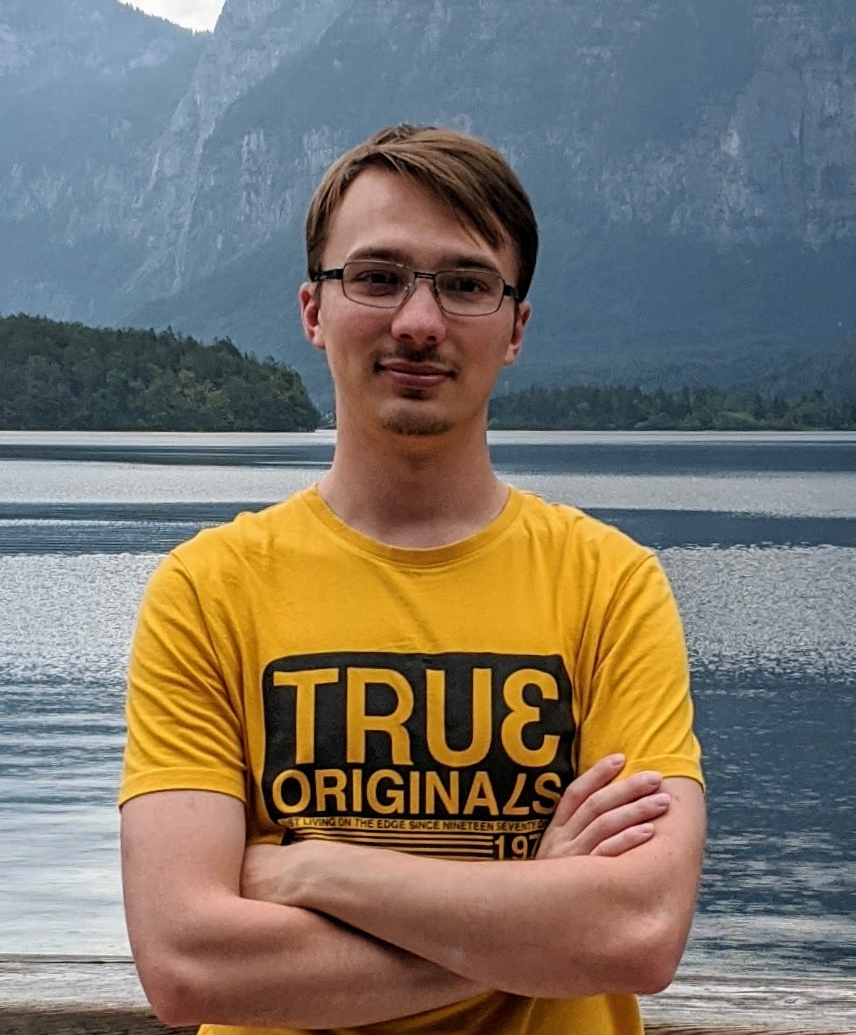
\includegraphics[width=\textwidth]{profile}
    \end{figure}
    Arcadii Rubailo \newline
    Age: 25 August 20, 1995 \newline
    \begin{tabular}{ l l }
        \includesvg[height=20pt]{icon_flag}     &   \includesvg[height=12pt]{icon_flag_md} Moldova \\
        \includesvg[height=20pt]{icon_home}     &   \includesvg[height=12pt]{icon_flag_cz} Videnska 22, Brno \\
        \includesvg[height=20pt]{icon_phone}    &   +420 775 087 503 \\
        \includesvg[height=20pt]{icon_email}    &   rubailo.arcadii@gmail.com \\
        \includesvg[height=20pt]{icon_linkedin} &   /arcadii-rubailo \\
        \includesvg[height=20pt]{icon_github}   &   /elderanakain \\
        \includesvg[height=20pt]{icon_language} &   \begin{tabular}{ l l }
                                                        Russian & Native \\ \hline
                                                        English & C1 \\ \hline
                                                        Romanian & B1 \\ \hline
                                                        Czech & A1 \\ \hline
                                                    \end{tabular} \\
        \includesvg[height=20pt]{icon_list}     &   \textbf{\large{Skills}} \\
                                                &   Programming languages: \\
                                                &   Kotlin, Java. \\
                                                &   Development tools: \\
                                                &   Android Studio, \\
                                                &   IntelliJ IDEA, \\
                                                &   Zeplin, Jira, Figma. \\
    \end{tabular}
\end{minipage}
\hspace{15pt}
\begin{minipage}[t]{0.6\textwidth}
    \raisebox{-.25\height}{\includesvg[height=20pt]{icon_school}} Education
    
    \bigskip
    
    Masaryk University – MSc \hfill 2017 – 2019 \newline
    Faculty of Informatics \newline
    Service Science, Management and Engineering programme
    
    \bigskip
    
    State University of Moldova – BSc \hfill 2014 – 2017 \newline
    Mathematics and Computer Science \newline
    Computer science programme
    
    \bigskip
    
    \raisebox{-.25\height}{\includesvg[height=20pt]{icon_work}} Experience
    
    \bigskip
    
    Kiwi.com \hfill 07.2018 – Present \newline
    Kiwi.com Android app, booking main developer. \newline
    Tech stack: Kotlin/Java, MVVM, Realm, ARCore (OpenGL), \newline
    Dagger2/Koin, Databinding\&LiveData, Moshi/Gson, \newline
    RxJava2/Flow, Jetpack Libraries, Retrofit2+OkHttp3.
    
    \bigskip
    
    Ellation \hfill 01.2017 – 08.2017 \newline
    VRV and Crunchyroll Android apps development. \newline
    Tech stack: Java/Kotlin, Retrofit2+OkHttp3, Chromecast, MVP, \newline
    Fabric, Exoplayer, Firebase, Branch.io, Outbound.io, JUnit4, \newline
    Mockito1.
   
    \bigskip
    
    Yopeso \hfill 08.2016 – 01.2017 \newline
    limango Android app development. \newline
    Tech stack: Java, Retrofit+OkHttp3, Firebase, RxJava, MVP, \newline
    JUnit4+Mockito2, Dagger2, SQLite.
    
    \bigskip
    
    Travod International \hfill 10.2015 – 08.2016 \newline
    Technical support, DTP and project management. \newline
    Tech stack: Photoshop, InDesign, SDL Trados.
    
    \bigskip
    
    Aursoft \hfill 02.2015 – 12.2015 \newline
    MyBebe Android app development. \newline
    Tech stack: Java, Support Library, Volley, Picasso, SQLite.

    \bigskip
    
    Hobbies and interests
    
    \bigskip
    
    Reading: science fiction, IT blogs, self-development. Master of sports in archery.
\end{minipage}\\
\end{document}
